% Chapter 1

\chapter{Introduzione} % Write in your own chapter title
\label{Chapter1} 
\lhead{\emph{Introduzione}}

%\section{Scopo del progetto}
%\label{sec:sec_scopoProgetto}

Questa relazione illustra il progetto del layout di un circuito sommatore CMOS integrato che sfrutti la tecnica TSPC (\textit{True Single Phase Clock}) presentata da \textit{Yuan} e \textit{Svensson} nell'articolo (CITA ARTICOLO). Il lavoro si inserisce nell'ambito del corso di Microelettronica tenuto dal Prof. Daniele Caviglia nella Laurea Magistrale in Ingegneria Elettronica dell'Università degli Studi di Genova.

L'elaborato vuole descrivere nel dettaglio il lavoro svolto, i risultati raggiunti e le problematiche riscontrate durante lo stesso. Inizieremo dunque con l'illustrare i vari passi percorsi, per poi scendere nel dettaglio delle fasi di analisi (sia della tecnologia utilizzata che del circuito sommatore) e di progettazione vera e propria.

\section{Fasi di lavoro}
\label{sec:sec_fasiLavoro}

In Fig. \ref{fig:workflow} è rappresentato il diagramma di flusso che abbiamo seguito durante il nostro lavoro. Tale sequenza di passi è generalizzabile a qualsiasi progetto di circuiti digitali, quando si parte da uno schema circuitale e si vuole giungere al disegno delle maschere di produzione che lo realizzano. Nel diagramma ogni rettangolo indica l'operazione da eseguire, mentre il rombo comporta un controllo che determina il passo successivo da intraprendere. 

\begin{figure}[hbt!]
	\centering
	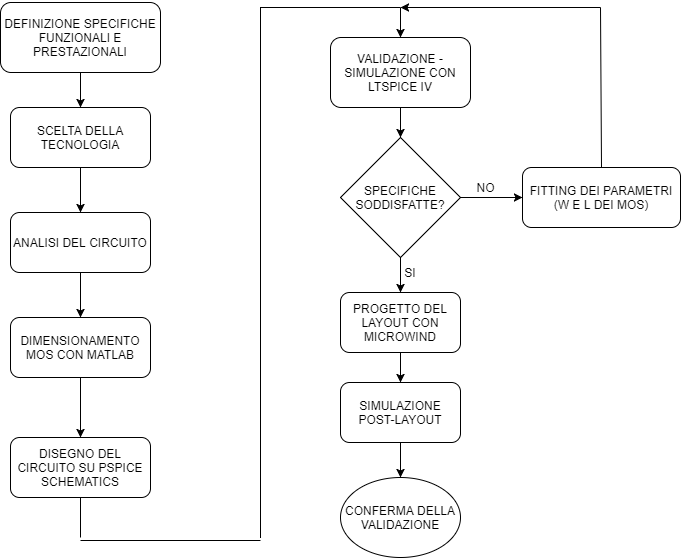
\includegraphics[width=1\textwidth]{figure/WorkflowDiagram.png}
	\caption{Flusso di progetto.}
	\label{fig:workflow}
\end{figure}

Prima di scendere nel dettaglio delle varie fasi introduciamo i vari software utilizzati nel corso del progetto. Già indicati nel diagramma di flusso, essi sono:

\begin{itemize}
	\item \textit{MATLAB}: software che facilita l'esecuzione e la gestione di calcoli matematici;
	\item \textit{PSpice}: programma di simulazione circuitale;
	\item \textit{LTspice IV}: anch'esso dedicato alla simulazione circuitale, lo abbiamo scelto in quanto il precedente PSpice nella versione gratuita presenta alcune restrizioni, in particolare sul numero massimo di transistor presenti nel circuito;
	\item \textit{Microwind}: software per il disegno di maschere di produzione di circuiti integrati.
\end{itemize}

Procediamo quindi con la descrizione del flusso di progetto di Fig. \ref{fig:workflow} in relazione al nostro lavoro. Il punto di partenza è la definizione delle specifiche di progetto. Queste nel nostro caso ci sono state fornite come consegna e sono riassunte nel seguente elenco:

\begin{itemize}
	\item Tensione di alimentazione $V _{DD}$: 1.2 V
	\item Capacità di carico $C _{load}$ sulle uscite \textit{SUM} e \textit{CARRY}: 100 fF
	\item Frequenza operativa minima $f _{min}$: 2 GHz
	\item Tipologia di progettazione del circuito: \textit{standard cell}
	\item Segnali di ingresso: tre generatori di tensione ideali, con tempi di salita e di discesa pari a 25 $\mu s$
\end{itemize}

Anche il tipo di tecnologia ci è stato indicato nella consegna del progetto: tecnologia CMOS 0.12$\mu m$. Questo dato è molto importante nel progetto di circuiti integrati, in quanto tra le altre cose indica la lunghezza minima di canale che possono avere i transitor MOS.

La terza fase prevede l'analisi dello schema circuitale del Full Adder presente nell'articolo citato nell'introduzione. Nella sezione \ref{sec:mos} sarà illustrata l'analisi in dettaglio. A partire da quest'ultima, come vedremo, è stato possibile individuare le relazioni analitiche che ci hanno permesso di legare i nostri parametri di progetto, ottenuti a partire dalle specifiche funzionali e prestazionali, con i parametri liberi, ovvero le dimensioni dei transistor MOS presenti nel circuito. 

Il dimensionamento dei MOS è per l'appunto la quarta fase del processo e ne rappresenta uno dei momenti più critici, in quanto getta le basi per il funzionamento del circuito finale. Esso tuttavia è basato sull'utilizzo di modelli analitici approssimati, per cui le dimensioni dei MOS trovati a questo passo non sono quelle definitive. Nel cap. \ref{Chapter3}, dedicato alla progettazione circuitale, parleremo in dettaglio di questo aspetto.

Ottenuta una prima approssimazione delle dimensioni dei transistor si procede con la quinta fase, la quale prevede il disegno del circuito su un software che ne permetta la simulazione. In particolare noi abbiamo disegnato il circuito su PSpice Schematics, ne abbiamo esportato la netlist, e abbiamo simulato quest'ultima con LTspice IV, per i problemi di cui abbiamo già parlato. Anche questo passaggio sarà esaurientemente descritto nel cap. \ref{Chapter3}, impiegando per le simulazioni il modello del MOS fornito da Microwind e dipendente dalla tecnologia di processo scelta. 

Il passo successivo è uno dei più interessanti. La fase precedente ha infatti permesso di ottenere una simulazione del circuito dimensionato per via analitica, ma come abbiamo già detto non ci si deve stupire se il risultato non è soddisfacente. Occorre un'attenta analisi dei segnali presenti in ogni ramo del circuito così da individuare eventuali punti critici e perfezionare di conseguenza le dimensioni dei MOS. Inizia così una fase di \textit{fitting dei parametri}, composta da un ciclo di analisi e ritocco delle dimensioni, che termina soltanto quando ci si ritiene soddisfatti della simulazione circuitale. 

Identificate le dimensioni finali dei transistor si procede al progetto e disegno del layout di circuito su Microwind, secondo l'approccio \textit{standard cell}. Questa fase sarà descritta nel Cap. (CAP. LAYOUT) e, una volta terminata, è seguita da una simulazione finale post-layout che, se in accordo con la simulazione pre-layout, consente di validare il disegno finale. 








